\section{Exposition: \mk and Biased Conjunction}
\label{sec:exposition}

In this section we give a formal syntax for the language we will use in the rest of the paper. We also describe the intentions and common design
choices lying behind existing implementations and demonstrate on a number of examples the ``biased conjunction problem'' which we are going to attack.
As the material of this section serves mainly as a motivation we will not present a formal semantics for the language, which can be found in~\cite{fair:semantics},
and leave out the description of some subtleties.

The syntax of the language is shown in Fig.~\ref{syntax}. We conventionally define the set of terms $\mathcal{T}_\mathcal{X}$
over the constructors with arities $\mathcal{C}$ and \emph{syntactic} variables $\mathcal{X}$. Note, we keep the parameterization of $\mathcal{T}_\mathcal{X}$ by $\mathcal{X}$
explicit since later we will also use another its parameterization by the set of \emph{semantic} variables. We also define the set $\mathcal{R}$ of relation names with arities.

Next, we introduce the central construct of \mk~--- a goal $\mathcal{G}$. A goal is either a unification of terms, disjunction or conjunction of goals, introduction of fresh variable,
or an application of a relation to terms. Relation definition $\mathcal{D}$ corresponds to an abstraction of a goal over the set of arguments. Finally, a specification $\mathcal{S}$
puts a top-level goal in the context of a list of relation definitions.

In a nutshell, here we deal with a simple first-order language in which goals play a role of function bodies and ``\lstinline|fresh|''~--- additional binders. Thus,
conventional notions of free variables and substitutions of variables by terms in terms and goals come naturally.

From now on we stipulate that all specifications are well-formed, meaning that all relational names have unique definitions, none of the definitions has
free variables and all relation applications respect the arity of corresponding relation names. The only place where free variables can be encountered in specification
is its top-level goal, and the evaluation of this goal delivers all bindings (\emph{answers}) for these variables which satisfy the constraints imposed by the specification.

More concretely, a goal defines a search procedure which for a given \emph{state} returns a finite or infinite stream of states. For now we can assume that states are represented by
substitutions from variables to terms although in actual implementations they can hold some extra information needed, for example, for allocating fresh variables.
This procedure is defined inductively by case analysis on the shape of the goal (we denote current substitution as $\theta$):

\begin{itemize}
\item For unification $t_1 \equiv t_2$ an attempt to unify the terms $t_1\theta$ and $t_2\theta$ is made. On success the most general unifier is integrated into $\theta$ and the resulting substitution
  is returned as a one-element stream; otherwise an empty stream in returned.

\item For disjunction $g_1 \vee g_2$ the evaluation steps of $g_1\,(\theta)$ and $g_2\,(\theta)$ are taken in an alternating manner, and the results are collected in a common stream. This evaluation
  discipline~--- \emph{interleaving}~\cite{fair:interleaving}~--- provides the \emph{completeness} of \mk search: each answer will be found in a finite number of steps.

\item For conjunction $g_1 \wedge g_2$, first, the left conjunct $g_1\,(\theta)$ is fully evaluated. Then, for each element $\theta^\prime$ (if any) of the resulting stream $g_2\,(\theta^\prime)$ is
  evaluated, and all resulting streams are concatenated. Thus, the evaluation of conjunction is \emph{left-biased}: none of evaluation steps in $g_2$ are performed until the next answer for
  $g_1\,(\theta)$ is found.

\item For fresh variable introduction \lstinline|fresh ($x$) $\;g$| a new variable, not occurring anywhere in $\theta$, is chosen and substituted for $x$ in $g$. Then the resulting goal is evaluated.

\item For relation application $R^k\,(t_1,\dots,t_k)$ the corresponding definition $R^k=\lambda x_1\dots x_k\,.\,g$ is found and all variables $x_i$ are substituted by terms $t_i$ in
  $g$. Then the resulting goal is evaluated for $\theta$ (we assume no capturing occurs during the substitution).
\end{itemize}

\begin{figure}[t]
\[
  \begin{array}{rcll}
     \mathcal{C} & = & \{ C_1^{k_1}, C_2^{k_2}, \ldots \} 
     & \mbox{constructors with arities} 
     \\
     \mathcal{X} & = & \{x_1, x_2, \ldots \} 
     & \mbox{syntactic variables} 
     \\
     \mathcal{T}_\mathcal{X} & = & \mathcal{X} \mid C_i^{k_i}(\mathcal{T}_\mathcal{X}^1, \ldots, \mathcal{T}_\mathcal{X}^{k_i})
     & \mbox{syntactic terms} 
     \\
     \mathcal{R} & = & \{R_1^{k_1}, R_2^{k_2}, \ldots \} 
     & \mbox{relation names} 
     \\
     \mathcal{G} & =    & \mathcal{T}_\mathcal{X} \equiv \mathcal{T}_\mathcal{X} & \mbox{unification} \\
                 & \mid & \mathcal{G} \lor \mathcal{G} & \mbox{disjunction} \\
                 & \mid & \mathcal{G} \land \mathcal{G} & \mbox{conjunction} \\
                 & \mid & \mbox{\lstinline|fresh|} \; (\mathcal{X}) \; \mathcal{G} & \mbox{fresh variable introduction} \\
                 & \mid & R_i^{k_i}(\mathcal{T}_\mathcal{X}^1, \ldots, \mathcal{T}_\mathcal{X}^{k_i}) & \mbox{relation application} \\
    \mathcal{D} & = &R_i^{k_i} = \lambda \mathcal{X}_1 \ldots \mathcal{X}_{k_i}. \; \mathcal{G} & \mbox{relation definition}\\
    \mathcal{S} & = &\mathcal{D}_1\mathcal{D}_2\dots\mathcal{D}_k \diamond \mathcal{G} & \mbox{specification}
  \end{array}
\]
    \caption{The syntax of relational language}
    \label{syntax}
\end{figure}


It is easy to see that this implementation ideas give rise to a monadic framework over the set of streams with evaluation rules for conjunction and disjunction playing roles of ``bind'' and
``mplus'' respectively. In an actual implementation a few embellishments can be added to this general framework: for example, some evaluation steps can be deferred using so-called
\emph{inverse-$\eta$-delay}~\cite{MicroKanren}; in conjunction instead of left conjunct the right one can be chosen for evaluation first; various interleaving disciplines can
be applied to make the distribution of steps within a cluster of disjunctions more fair~\cite{fair:towardsAM}, etc. However, in all cases the basic implementation principles remain
the same.

We now consider a few examples of relational definitions and specifications. The following definition\footnote{By tradition, the names of relations are superscripted by ``$^o$''.}
introduces a relational list concatenation:

\begin{lstlisting}
  append$^o$ = $\lambda\; x\; y\; xy$ . ($x$ ===$\,$ [] /\ $y$ === $\;xy$) \/
                      fresh ($e\; xs\; xys$) 
                        $x\;$ === $\;e$ : $xs$ /\ 
                        $xy\;$ === $\;e$ : $xys$ /\ 
                        append$^o$ $xs\; y\; xys$
\end{lstlisting}

Three arguments $x$, $y$ and $xy$ correspond to three lists such that the concatenation of $x$ and $y$ equals $xy$. The relation is defined using case analysis and recursion: if
$x$ is empty (\lstinline|[]|) then $xy$ should be equal $y$; otherwise we split $x$ into a head $e$ and a tail $xs$ and set $y$ to \lstinline|$e$ : $xys$|, where
$xys$ is a concatenation of $xs$ and $y$, obtained via a recursive call to the same relation (we use here ``\lstinline|[]|'' and ``\lstinline|:|'' as constructor names).

In the context of this definition the top-level goal

\begin{lstlisting}
       append$^o$ [A] [B] $x$
\end{lstlisting}

would calculate a substitution

\[
x \mapsto \mbox{\lstinline|[A, B]|}
\]

which is an expected outcome. However, as unification actually works in both direction, the same relation can be used to solve other problems as well. For example

\begin{lstlisting}
       append$^o$ [A] $x$ [A, B]
\end{lstlisting}

gives us

\[
x \mapsto \mbox{\lstinline|[B]|}
\]

while

\begin{lstlisting}
       append$^o$ $x$ $y$ [A, B]
\end{lstlisting}

gives us a whole bunch of answers

\[
\begin{array}{ll}
  x \mapsto \mbox{\lstinline|[]|} & y \mapsto \mbox{\lstinline|[A, B]|} \\
  x \mapsto \mbox{\lstinline|[A]|} & y \mapsto \mbox{\lstinline|[B]|} \\
  x \mapsto \mbox{\lstinline|[A, B]|} & y \mapsto \mbox{\lstinline|[]|} 
\end{array}
\]

(not necessarily in this order). In other words, the same relation definition can be used to perform the search in various ``directions''~--- not only calculate
outputs for given inputs, but also vice versa, and, generally in any possible way depending on the distribution of free variables.

In all aforementioned examples the evaluation of a goal returned a finite stream. This is, however, not always the case. For example, if we put the recursive call in the definition of
\lstinline|append$^o$| \emph{first} in the conjunction, then the evaluation of the goal \lstinline|append$^o$ $x$ $y$ [A, B]| will \emph{diverge} after returning all the answers. We
can illustrate this behavior by the following diagram:

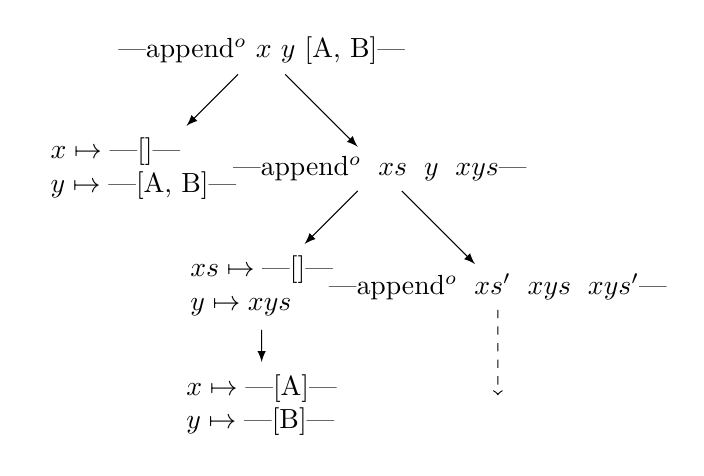
\begin{tikzpicture}[sibling distance=3cm,edge from parent/.style={draw,-latex}]
  \node{\lstinline|append$^o$ $x$ $y$ [A, B]|}
    child {
      node{$\begin{array}{l}
              x\mapsto\mbox{\lstinline|[]|}\\
              y\mapsto\mbox{\lstinline|[A, B]|}
            \end{array}$}
    }
    child {
      node{\lstinline|append$^o\;$ $xs\;$ $y\;$ $xys$|}
        child {
          node{$\begin{array}{l}
                  xs\mapsto\mbox{\lstinline|[]|}\\
                  y\mapsto xys
                \end{array}$}
            child {
              node{$\begin{array}{l}
                      x\mapsto\mbox{\lstinline|[A]|}\\
                      y\mapsto\mbox{\lstinline|[B]|}
                    \end{array}$}
            }
        }
        child {
          node{\lstinline|append$^o\;$ $xs^\prime\;$ $xys\;$ $xys^\prime$|}
             child {
                node{} edge from parent[->, dashed]
            }
        } 
    };
\end{tikzpicture}

Here the left and right branches of nodes correspond to the evaluation of the first and the second disjuncts of \lstinline|append$^o$| respectively. We start from
the first disjunct of the topmost \lstinline|append$^o$| application which immediately gives us the first answer $x\mapsto\mbox{\lstinline|[]|},\,y\mapsto\mbox{\lstinline|[A, B]|}$.
In the second disjunct we encounter a conjunction and start to evaluate its left conjunct, which is an application of \lstinline|append$^o$| to \emph{free} variables
$xs$, $y$, and $xys$. Recursing in the body, we again encounter a disjunction. Its left disjunct gives us the substitution $xs\mapsto\mbox{\lstinline|[]|},y\mapsto xys$ which, upon 
returning from the recursive call and evaluating the remaining conjuncts, gives us the second answer $x\mapsto\mbox{\lstinline|[A]|},y\mapsto\mbox{\lstinline|[B]|}$. The right
disjunct, however, is again a conjunction starting with the recursive application of \lstinline|append$^o$| to (some other) free variables. Clearly, this branch will never stop to
grow, and, after recovering the third answer, the evaluation will diverge. This example demonstrates a well-known phenomenon of \emph{refutational incompleteness}~\cite{fair:WillThesis}
of this specific implementation of \lstinline|append$^o$|. It can be proven~\cite{fair:semantics} that the initial implementation (with the recursive call placed last in the conjunction)
is refutationally complete, but only for \emph{linear} applications (i.e. applications in which no variable occurs in the argument terms more than once).

Pushing relation application to the end in the cluster of conjunctions is a well-known trick in relational programming, which often helps to improve the performance or even
convergence of goal evaluation. This trick, however, does not help in all cases~--- for example, when there are more then one application in a cluster. Consider, for instance, the
following relation \lstinline{revers$^o$}, which associates an arbitrary list with the list containing the same elements in the reverse order:

\begin{lstlisting}
  revers$^o$ = $\lambda\;x\;y\;$ . ($x$ === $\;$[] /\ $y$ === $\;$[]) \/
                    fresh ($e\; xs\; ys$) 
                       $x$ === $\;e$ : $xs$ /\ 
                       revers$^o$ $xs$ $ys$ /\
                       append$^o$ $ys$ [$e$] $y$
\end{lstlisting}

In this relation there are two applications in the same conjunction: \lstinline{revers$^o$} and \lstinline{append$^o$}; thus, it is impossible to put both of them last. With this particular
order of applications the goal \lstinline|revers$^o$ [A, B, C] $x$| converges, but with the reverse order the same goal diverges after the answer is found. Moreover, the reverse order negatively
affects the performance of answer evaluation. At the same time the goal \lstinline|revers$^o$ $x$ [A, B, C]| demonstrates the symmetric behavior: it diverges for the given order of conjuncts,
and converges for the reverse one.

An important design goal for \mk was to provide a purely declarative way to define executable relational specifications which would work equally well regardless of the ``direction'' of the search.
In particular, as we expect conjunction and disjunction to be commutative and associative, the order of conjuncts/disjuncts must not have a notable impact on the behavior of
a specification. As these examples demonstrate, this goal is not completely achieved yet. More interestingly, all these cases are the manifestations of the same flaw in conventional
relational search strategy~--- the \emph{left-bias} in conjunction evaluation. We demonstrate this by the following artificial example. First, we define two relations \lstinline{div$^o$} and
\lstinline|fail$^o$| as follows:

\begin{lstlisting}
  div$^o$  = $\lambda\;x$ . div$^o\;$ x
  fail$^o$ = $\lambda\;x$ . A === $\;$B
\end{lstlisting}

In both cases the argument $x$ is a ``phony'' parameter. Clearly, \lstinline|div$^o$| diverges with no answers, while \lstinline|fail$^o$| in one step evaluates to an empty stream (\emph{fails}). Thus,
one would expect the conjunction of these relations to fail in one step. Indeed, the conjunction

\begin{lstlisting}
  fail$^o$ _ /\ div$^o$ _
\end{lstlisting}

fails, but the symmetrical one

\begin{lstlisting}
  div$^o$ _ /\ fail$^o$ _ 
\end{lstlisting}

diverges with no answer (here underscore denotes some irrelevant term). The explanation is trivial~--- during conjunction evaluation we first evaluate its left conjunct
until the first answer is found. In the first case we immediately come up with an empty stream, and the evaluation of the whole conjunction fails. In the second case,
however, we never get an answer; at the same time we always have some remaining steps to be performed in the evaluation of the left conjunct, which means that the
whole search diverges. This behavior of conjunction not only leads to a divergence in some important cases~--- it also heavily impacts the performance by polluting
the search tree with never ending branches, which at the same time do not produce any results. In some cases this can be avoided by adjusting the order of conjuncts in
the relation definition to fit a certain evaluation direction, but, as shown in~\cite{fair:DivTest}, the solution of some problems require the same definition to be run in
various direction at the same time. Thus, in the general case, under biased conjunction evaluation strategy no optimal static order of conjuncts exists.


%We propose a completely different evaluation strategy for conjunction which dynamically postpones the evaluation of some branches using runtime analysis of
%intrinsic properties of relations being evaluated. 

\begin{comment}
The main syntactic notion of \mk is \textbf{goal}. There are only four syntactic forms of goals.

\begin{itemize}
\item[$\bullet$] Unification~\cite{fair:unify} $t_1 \equiv t_2$, where $t_1, t_2$ are some terms that contain constructors and variables. Unification is the basic
  construct to create goals. If $t1, t2$ are unified, then the goal is considered successful. In this case the result of unification is a singleton stream which
  contains the most common unifier of $t_1, t_2$. Otherwise, the goal is failed and result is empty stream.
\item[$\bullet$] Disjunction $g_1 \lor g_2$, where $g_1, g_2$ are some goals. Both goals are evaluated independently. The result of disjunction is the union of answers for $g_1$ and $g_2$.
\item[$\bullet$] Conjunction $g_1 \land g_2$, where $g_1, g_2$ are some goals. First, we evaluate the goal $g_1$, and then we evaluate the goal $g_2$ in the context of each
  answer for $g_1$. As a result, we get answers for both $g_1$ and the $g_2$ simultaneously.
\item[$\bullet$] Fresh variable introduction \!$\lstinline{fresh} (x). \, g$, where $x$ is a variable and $g$ is a goal. This construct is used to introduce a fresh variable $x$
  to be used in the goal $g$.
\end{itemize}

The result of \mk program evaluation is a lazy, possibly infinite stream of answers, represented as substitutions.

As an example we consider a relational definition of list concatenation (Fig.~\ref{fair:lst-appendo}). The relation \lstinline|append$^o$ x y xy| can be interpreted as the following:
the concatenation of lists \lstinline|x| and \lstinline|y| equals list \lstinline|xy|.

\begin{figure*} %[h!]
\centering
\begin{tabular}{c}
\lstinline|fresh (x) (append$^o$ [1] [2] x)| $\Rightarrow$ \lstinline|{x = [1,2]}| \\
(a) \\[5mm]
\lstinline|fresh (x) (append$^o$ [1] x[1,2,3])| \!$\Rightarrow$ \lstinline|{x = [2,3]}|\\
(b) \\[5mm]
\lstinline|fresh (x y) (append$^o$ x y[1,2])| $\Rightarrow \left\{
\begin{array}{ll}
\mbox{\lstinline{x = [],}}    & \mbox{\lstinline{y = [1,2];}} \\
\mbox{\lstinline{x = [1],}}   & \mbox{\lstinline{y = [2];}} \\
\mbox{\lstinline{x = [1,2],}} & \mbox{\lstinline{y = []}} \\
\end{array} \right\}$ \\
(c) \\[5mm]
\lstinline|fresh (x y) (append$^o$ x [1] y)| $\Rightarrow \left\{
\begin{array}{ll}
\mbox{\lstinline{x = [],}}    & \mbox{\lstinline{y = [1];}} \\
\mbox{\lstinline{x = [}} \alpha_1\! \mbox{\lstinline{],}} & \mbox{\lstinline{y = [}} \alpha_1\! \mbox{\lstinline{,1];}} \\
\mbox{\lstinline{x = [}} \alpha_1, \alpha_2\! \mbox{\lstinline{],}} & \mbox{\lstinline{y = [}} \alpha_1, \alpha_2\! \mbox{\lstinline{,1];}} \\
...
\end{array} \right\}$ \\
(d)\\[5mm]
\lstinline|fresh (a x) (append$^o$ [a] x [])| $\Rightarrow$ \lstinline|{}|\\
(e) 
\end{tabular}
\caption{Examples of relation \lstinline|append$^o$|}
\label{fair:appendo-examples}
\end{figure*}

We consider a few different queries for the relation \lstinline|append$^o$| (Fig.~\ref{fair:appendo-examples}). First of all, we can concatenate two lists
(Fig~\ref{fair:appendo-examples}a). Also we can find a list suffix (Fig.~\ref{fair:appendo-examples}b). Moreover, we can synthesize a finite stream of all
list pairs which, being concatenated, deliver given result (Fig.~\ref{fair:appendo-examples}c) or an infinite stream of all lists with a given suffix (Fig.~\ref{fair:appendo-examples}d).
Finally, we can prove some properties of relations. In particular, a singleton list is not a prefix of an empty list (Fig.~\ref{fair:appendo-examples}e).

\subsection{Directed Conjunction}

% В языке miniKanren между операциями дизъюнкции и конъюнкции есть существенная разница. Дизъюнкция вычисляет свои аргументы попеременно, что приводит к равномерному вычислению двух дизъюнктов. Такого поведения дизъюнкции достаточно для полного поиска ответов. Конъюнкция же извлекает ответы из первого конъюнкта, на которых вычисляет второй конъюнкт. С одной стороны, такая конъюнкция проста в реализации и позволяет явно задать порядок исполнения конъюнктов. С другой стороны, эта конъюнкция ассиметрична. Более того, она может сходиться при одном порядке конъюнктов, но расходиться при другом. Например, отнонение freeze в зависимости от аргумента либо сходится за один шаг рекурсии, либо расходится. Тогда конъюнкция вида (=== /\ freeze) сходится, но при перестановке конъюнктов мы получаем расхождение. Действительно, в первом случае первый конъюнкт производит ровно один ответ, который противоречит унификации в теле отношения freeze. Во втором случае отношение freeze разойдется и не произведет ни одного ответа и второй конъюнкт вычислен не будет. 

In \mk there is a significant difference between disjunction and conjunction evaluation strategy. The arguments of disjunction are evaluated
in an \emph{interleaving}~\cite{fair:interleaving} manner, switching elementary evaluation steps between disjuncts, which provides the completeness of the search.
Conjunction, on the other hand, waits for the answers from the first conjunct and then calculates the second conjunct in the context of each answer.

On the one hand, this strategy is easy to implement and allows one to explicitly specify the order of evaluation when this order is essential.
On the other hand, the strategy amounts to non-commutativity: the convergence of a conjunction can depend on the order of its arguments.
For example, the relation

\begin{lstlisting}
   let rec freeze$^o$ x = x ===  true /\ freeze$^o$ x
\end{lstlisting}

\noindent either converges in one recursion step or diverges. The conjunction \linebreak
\lstinline{(x === false/\ freeze$^o$ x)} converges, but the same conjunction with the reverse order of conjuncts
\lstinline{(freeze$^o$ x /\ x === false)} diverges. Indeed, in the first case the first conjunct produces exactly one answer which contradicts the unification in the body
of \lstinline{freeze$^o$}. In the second case the relation \lstinline{freeze$^o$} diverges and does not produce any answer. As a result we will never begin to evaluate the second conjunct.

\begin{figure}[h!]
\centering
\begin{tabular}{c}
%\begin{lstlisting}[firstnumber=7,numbers=left,numberstyle=\small,escapeinside={@}{@}]
%\begin{lstlisting}[firstnumber=7,numbers=left,numberstyle=\small,escapeinside={@}{@}]
\begin{lstlisting}[escapeinside={@}{@}]
let rec revers$^o$ x y =
  (x === [] /\ y === []) \/
  fresh (e xs ys) (
    x === e : xs /\ 
@\label{fair:reverso-call}@    revers$^o$ xs ys /\
@\label{fair:appendo-call}@    append$^o$ ys [e] y)
\end{lstlisting}
\end{tabular}

\caption{Relational list reversing}
\label{fair:lst-reverso}
\end{figure}

% Конечно, данная проблема решается правилом, которому нужно следовать при работе с miniKanren: унификацию нужно ставить самым левым конъюнктом. Но иногда оба конъюнктв являются вызовами отношений. В частности отношение обращения списка revers, которое связывает произвольный список со списком, содержащим элементы в обратном порядке. В этом отношении есть пара конъюнктов append и revers. При таком порядке вызов revers сходится, но при обратном порядке он расходится. Более того при обратном порядке снижается скорость вычисления ответа. 
The problem in this particular example can be alleviated by using a conventional rule for \mk, which says that unifications must be moved first in a cluster of conjunctions.
But the rule does not work for clusters with more than one relational call. Consider, for instance, the relation \lstinline{revers$^o$} (Fig.~\ref{fair:lst-reverso}), which associates
an arbitrary list with the list containing the same elements in reverse order. In this relation we can see a couple of conjuncts: \lstinline{revers$^o$} on line~\ref{fair:reverso-call} and
\lstinline{append$^o$} on line~\ref{fair:appendo-call}. With this particular order, the call \lstinline{(revers$^o$ [1, 2, 3] q)} converges, but in reverse order it diverges after an answer
is found. Moreover, the reverse order negatively affects the performance of the answer evaluation.

% В то же время, вызов revers при заданном порядке конъюнктов расходится, а при обратном сходится. В результате мы бы хотели разный порядок конъюнктов в зависимости от конкретных аргументов.

At the same time the call \lstinline{(revers$^o$ q [1, 2, 3])} for a given order of conjuncts diverges, and for the reverse order it converges. As a result a
different order of conjuncts is desirable depending on their runtime values.

% В следующих разделах мы предлжожим подход, который будет определять оптимальный порядок автоматически во время исполнения программы.
In the following sections we describe an approach for automatically determining a ``good'' order during program evaluation.
\end{comment}
